\subsection{Парабола}
\term{Парабола}~--- геометрическое место точек, равноудалённых от данной прямой (называемой \term{директрисой} параболы) и данной точки (называемой \term{фокусом} параболы).

\begin{wrapfigure}[11]{l}{0.5\tw}
	\centering
	\vspace{-.7pc}
	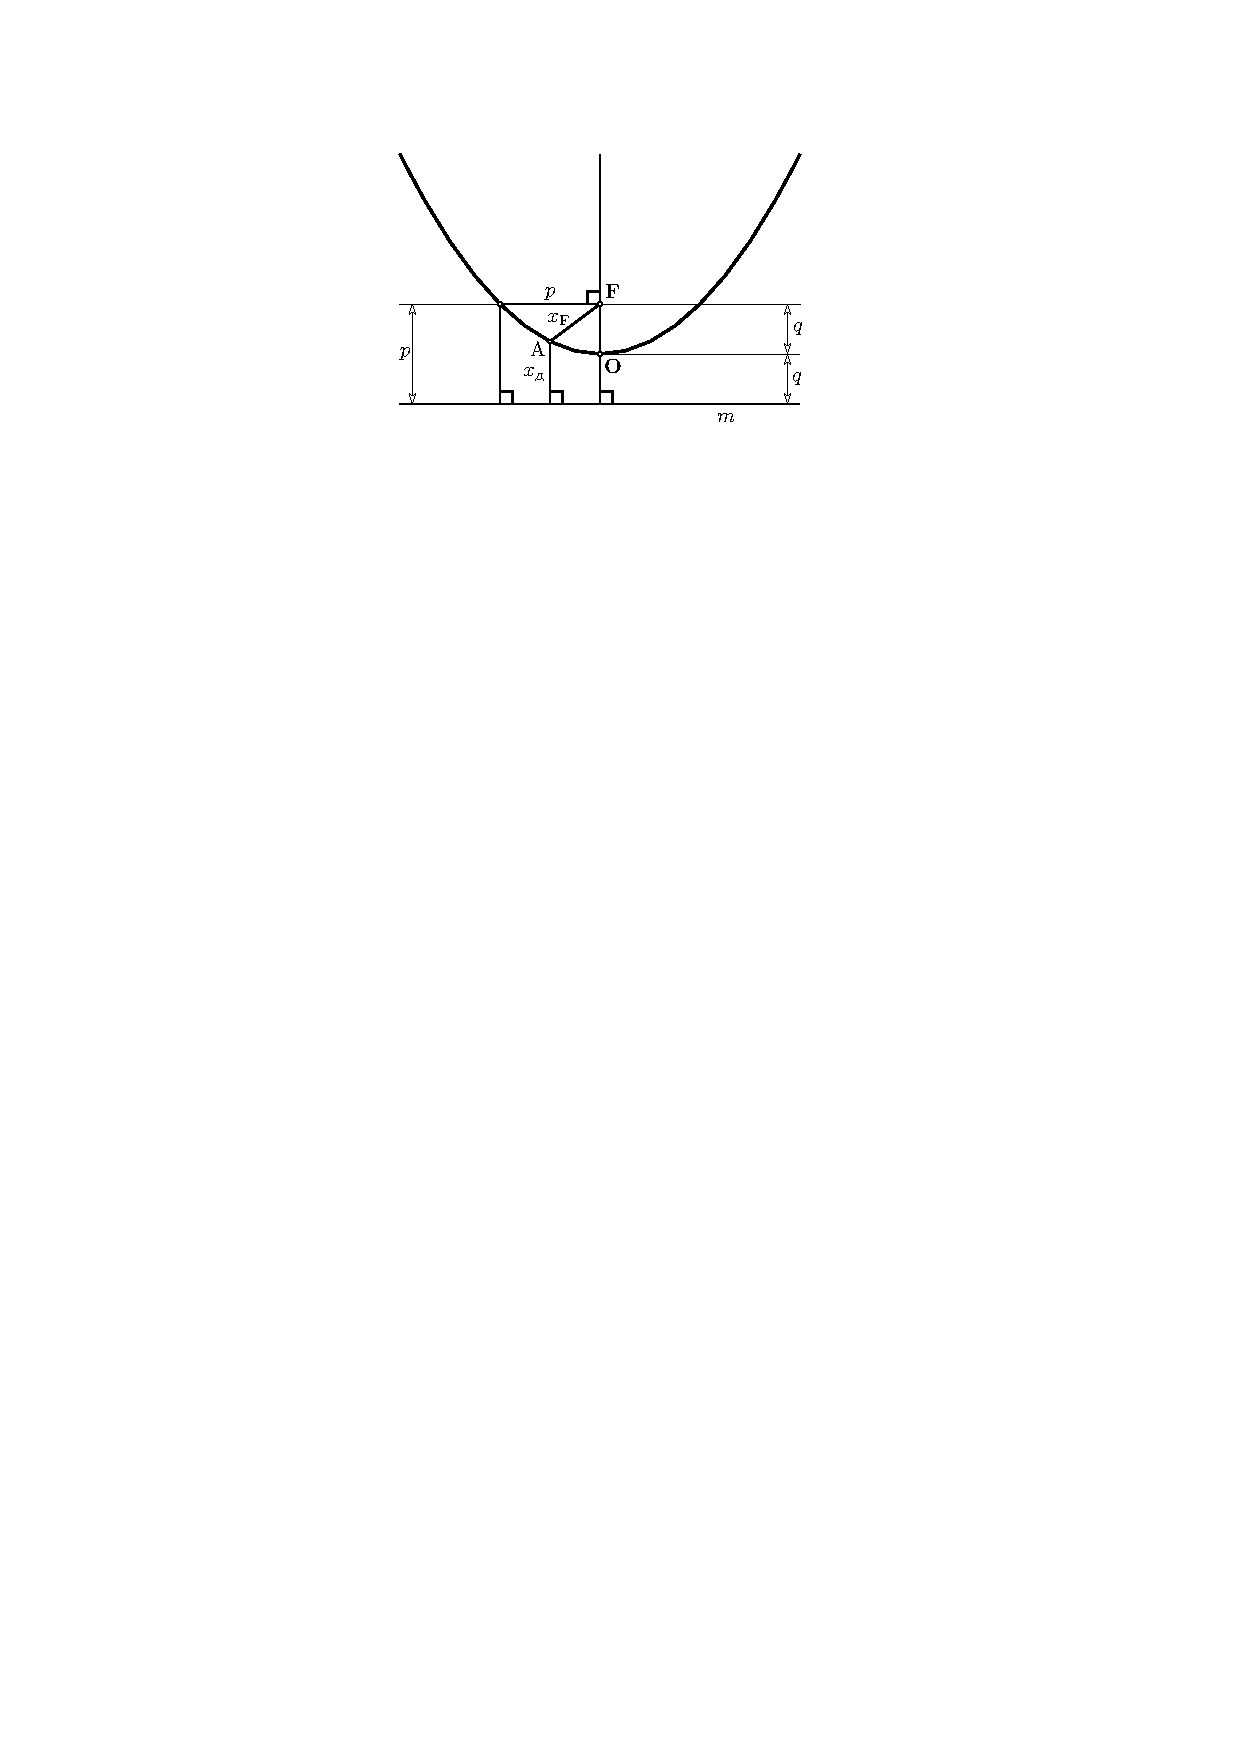
\includegraphics[width = 0.5\tw]{Parabola}
	\captionof{figure}{Парабола \label{pic:the-pic}}
\end{wrapfigure}
Получим из определения параболы её уравнение в декартовых координатах. Пусть расстояние между фокусом и директрисой параболы равно $p$. Из определения ясно, что существует точка параболы $P$, располагающаяся в середине перпендикуляра, опущенного из фокуса на директрису. Расположим параболу так, чтобы эта точка оказалась в начале координат. Тогда директриса будет задаваться уравнением $x = -p/2$, а фокус будет иметь координаты $(p/2, 0)$.

Приравняем теперь расстояния от произвольной точки параболы $(x, y)$ до фокуса и до директрисы:
\begin{gather*}
	x + \frac{p}{2} = \sqrt{\left(x - \frac{p}{2} \right)^2 + y^2},\\
	x^2 + \frac{p^2}{4} + px = x^2 + \frac{p^2}{4} - px + y^2,\\
	y^2 = 2px. \tag{\theequation}
\end{gather*}

В силу симметрии, перпендикуляр, опущенный из фокуса на директрису, является осью параболы, а точка $P$~--- её вершиной.

Легко заметить, что длина перпендикуляра, опущенного из фокуса на параболу, равна $p$. Этот отрезок называется \term{фокальным параметром}, а его длина, как следует из вышесказанного, равна расстоянию от фокуса до директрисы.

\begin{wrapfigure}[8]{r}{0.4\tw}
	\centering
	\vspace{-1pc}
	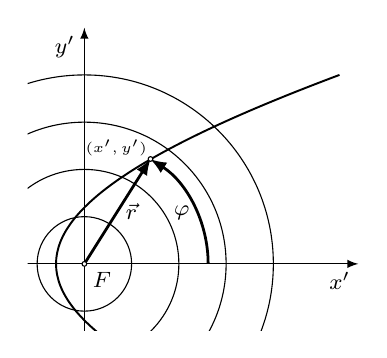
\begin{tikzpicture}[scale=1.2]
		\footnotesize
		\clip (-.3, -0.7) rectangle + (3.5, 3.2);
		
		\coordinate (xy) at (1, 1.11) {};
		\coordinate (F) at (.3, 0) {};
		
		\draw [line width = .7pt](3, 2) .. controls (-1, .5) and (-1, -.5) .. (3, -2);
		
		\draw [-latex] (.3, -2.2) -- (.3, 2.5);
		\draw [-latex] (-1, 0) -- (3.2, 0);
		
		\draw (F) circle (.5);
		\draw (F) circle (1);
		\draw (F) circle (1.5);
		\draw (F) circle (2);
		\draw (1.61, 0) [-latex, line width=1pt] arc (0:57.8:1.31);
		\draw [-latex, line width=1pt] (.3, 0) -- (1, 1.11);
		
		\draw (1.05, 1.05) node [anchor=south east] {\tiny{$(x', y')$}};
		\draw (F) node [anchor=north west] {$F$};
		\draw (.65, .55) node [anchor=west] {$\vec r$};
		\draw (1.5, .7) node [anchor=north east] {$\boldsymbol{\varphi}$};
		\draw (3.2, 0) node [anchor=north east] {$x'$};
		\draw (-.1, 2.5) node [anchor=north west] {$y'$};
		
		\draw (F) [fill=white] circle(.025);
		\draw (xy) [fill=white] circle(.025);
	\end{tikzpicture}
	
	\caption{}
\end{wrapfigure}
Перенесем теперь фокус параболы в начало координат и получим её уравнение в полярных координатах. Для этого нужно сделать такую замену: $x' \hookrightarrow x - p/2$, значит $x \hookrightarrow x' + p/2$, а $y' \hookrightarrow y$. Запишем теперь уравнение параболы:
\begin{gather*}
	y^2 = 2px,\\
	(y')^2 = 2 p \left(x' + \frac{p}{2} \right).
\end{gather*}
Перейдем теперь в полярные координаты:
\begin{gather*}
	r^2 \sin^2 \varphi = p^2 + 2pr\cos \varphi,\\
	r^2 \cdot \sin^2 \varphi - r \cdot 2 p  \cos \varphi - p^2,\\
	D = 4p^2 \cos^2 \varphi + 4 p^2 \sin^2 \varphi = 4 p^2,\\
	r = \frac{2p \cos \varphi \pm 2p}{2\sin^2 \varphi}, \quad r \geqslant 0,\\
	r = \frac{p (\cos \varphi + 1)}{1 - \cos^2 \varphi} = \frac{p (\cos \varphi + 1)}{(1 - \cos\varphi)(1 + \cos\varphi)} = \frac{p}{1 - \cos \varphi}.
\end{gather*}
Если же параболу развернуть на $180^\circ$, в знаменателе будет знак плюс. Это завершает вывод уравнения параболы в полярных координатах:
\begin{equation}
	r = \frac{p}{1 \pm \cos \varphi}.
\end{equation}

\begin{wrapfigure}{r}{0.45\tw}
	\centering
	\vspace{-.5pc}
	\begin{tikzpicture}[scale=1.2]
		\footnotesize
		\clip (-.4, -1) rectangle + (4, 3.5);
		
		\coordinate (xy) at (1, 1.11) {};
		\coordinate (F) at (.3, 0) {};
		
		\draw [line width = .7pt](3, 2) .. controls (-1, .5) and (-1, -.5) .. (3, -2);
		
		\draw [-latex] (0, -2.2) -- (0, 2.5);
		\draw [-latex] (-1, 0) -- (3.5, 0);
		
		\draw [-latex, line width=1pt] (F) -- (xy);
		\draw [-latex, line width=1pt] (xy) -- (2, 1.11);
		\draw [-latex, line width=1pt] (xy) -- (2, 1.67);
		\draw (xy) -- (3, 1.11);
		\draw [dashes] (3, 2.21) -- (-.5, 0.29);
		
		\draw (1.2, 1.11) node [anchor=south east] {$(x, y)$};
		\draw (F) node [anchor=north] {$F$};
		\draw (.65, .55) node [anchor=west] {$\vec r$};
		\draw (1.5, 1.11) node [anchor=north] {$\vec x$};
		\draw (1.5, 1.39) node [anchor=south] {$\vec t$};
		
		\draw (3.5, 0) node [anchor=north east] {$x$};
		\draw (0, 2.5) node [anchor=north west] {$y$};
		
		\draw (F) [fill=white] circle(.025);
		\draw (xy) [fill=white] circle(.025);
	\end{tikzpicture}
	
	\caption{}
\end{wrapfigure}
Как и все конические сечения, парабола обладает \imp{оптическим свойством}, которое формулируется следующим образом: пучок лучей, параллельных оси параболы, отражаясь в параболе, собирается в её фокусе. И наоборот, свет от точечного источника, находящегося в фокусе, отражается параболой в пучок параллельных её оси лучей.

Аналогично доказательству оптического свойства эллипса рассмотрим случай только верхней ветви. И выберем на ней произвольную точку $(x, y)$. Тогда вектор, определяющий направление луча из фокуса в выбранную точку задается вектором $\vec r = (x - p/2, y)$. Направление, соответствующее оси параболы, зададим единичным вектором $\vec x = (1, 0)$, так как ось параболы с каноническим уравнением совпадает с осью абсцисс. Остается только найти вектор касательной $\vec t$ в точке $(x, y)$. Для верхней ветви параболы каноническое уравнение эквивалентно $y = \sqrt{2px}$. Найдем производную данной функции:
\begin{gather*}
	y' = \frac{2p}{2\sqrt{2px}} = \sqrt{\frac{p}{2x}}.
\end{gather*}
Значит направляющий вектор касательной можно представить в виде
\begin{equation*}
	\vec t =
	\begin{pmatrix}
		1\\
		y'_x
	\end{pmatrix} =
	\begin{pmatrix}
		1\\
		\sqrt{\dfrac{p}{2x}}
	\end{pmatrix}.
\end{equation*}

Остается проверить равенство косинусов углов между векторами $\vec r$ и $\vec t$ и векторами $\vec x$ и $\vec t$:
\begin{gather*}
	\frac{\scalar{r}{t}}{|\vec r| | \vec t|} = \frac{\scalar{x}{t}}{|\vec x| |\vec t|},\\
	\scalar{r}{t} = |\vec r| \scalar{x}{t},\\
	\left(x - \frac{p}{2}\right)\cdot 1 + y \cdot \sqrt{\frac{p}{2x}}  = \sqrt{\left( x - \frac{p}{2} \right)^2 + y^2 } \left(1 \cdot 1 + 0 \cdot \sqrt{\frac{p}{2x}} \,\right),\\
	\left(x - \frac{p}{2}\right)^2 + \frac{y^2 p}{2x} + 2 y \cdot \sqrt{\frac{p}{2x}} \left(x - \frac{p}{2}\right) = \left(x - \frac{p}{2}\right)^2 + y^2,\\
	2  \sqrt{\frac{p}{2x}} \left(x - \frac{p}{2}\right) =  y \left( 1 - \frac{p}{2x} \right),\\
	\sqrt{\frac{4x^2p}{2x}} \left(1 - \frac{p}{2x}\right) =  y \left( 1 - \frac{p}{2x} \right),\\
	\sqrt{2xp}  =  y.
\end{gather*}
Получено уравнение верхней ветви параболы, которому, очевидно, координаты точки, принаблежащей параболе, удовлетворяют. Следовательно, оптическое свойство доказано.

Покажем, что парабола является коническим сечением. Для этого рассмотрим каноническое уравнение конической поверхности
\begin{equation*}
	\frac{x^2}{a^2} + \frac{y^2}{b^2} - \frac{z^2}{c^2} = 0
\end{equation*}
и секущую плоскость, параллельную образующей конуса и задаваемую уравнением
\begin{equation*}
	z = \frac{c(x + d)}{a},
\end{equation*}
где коэффициенты $a, b, c$ определяют вид поверхности, а $d$~--- положение плоскости. Подставим второе в первое:
\begin{gather*}
	\frac{x^2}{a^2} + \frac{y^2}{b^2} = \frac{x^2 + d^2 + 2yd}{a^2},\\
	\frac{y^2}{b^2} = \frac{d^2 + 2xd}{a^2},\\
	y^2 = 2 x \underbrace{\frac{b^2d}{a^2}}_p + \frac{d^2}{a^2 b^2}.
\end{gather*}
С точностью до вертикального сдвига получили каноническое уравнение параболы, что подтверждает принадлежность параболы множеству конических сечений.

